\clearemptydoublepage
\chapter{Background}

\chaptermark{Background}
%What is model driven engineering
%Metamodeling: definition and tools
%Main concepts: metamodel, constraint, transformation,
%Automation in MDE
%Evolution in MDE
In this chapter, we introduce the field of Model-Driven engineering. In section ?, we present the activity of metamodeling and the involved artifacts. Section ? discusses the automation task related to the artifacts presented in section ?. We finish this chapter with a presentation of the evolution concept in the context of model driven engineering.
%define the terminology of the main concepts that we use. 
% We define the specific scope of problems addressed in this thesis
% and discuss the spectrum of problems that arise in this field. 
%TODO Terminology: Model-Driven engineering, co-evolution
% Metamodel, co-evolution, code, maintenance, refactoring

\section{Model-Driven Engineering}
To develop a software, a list of specifications is given to the developers, to code the final product. This approach can work in the case of small projects. When the complexity of the software increases, more efficient approaches must be adopted. Model driven engineering has proven  its efficiency comparing to other engineering disciplines \cite{1231146}.

%\boitemagique{Model-Driven Enginereering}{
\textit{Model-Driven Engineering(MDE)} is the systematic use of models as primary artifacts during a software engineering process. MDE includes various model-driven approaches to software development, including model-driven architecture, domain-specific modeling and model-integrated computing~\cite{10.1145/1985793.1985882}. The first appearance of MDE like approaches started in the 80's \cite{10.1007/s10270-005-0079-0}. MDE is still adopted  and a lot of work is being done in academia and industry, refs.
//improve communication between multi-disciplinary collaborators.

%}
%TODO detaills the benefits of MDE

%Details about MDE approach 
The goal of MDE is to improve productivity, quality, and maintainability by leveraging high level abstractions throughout the development process. The metamodeling phase implied the experts of the domain who focus on the major key aspects of the problem rather than being concerned about the underlying programming language and the implementation.
%about major key aspects of the problem statement rather than focusing on programming.
%Metamodeling and modeling langugaes

% MEtamodel def :
The metamodel represent the main artifact in MDE. There are many definitions of the concept "metamodel" that can be found in literature \cite{stahl2006model}:

\textit{A metamodel} describes concepts that can be used for modeling the model (i.e. in the instances of the metamodel).

\textit {Metamodels} are models that make statements about modeling. More precisely, a metamodel describes the possible structure of models in an abstract way, it defines the constructs of a modeling language and their relationships, as well as constraints and modeling rules, but not the concrete syntax of the language.

\textit{A metamodel} defines the abstract syntax and the static semantics of a modeling language ,Vice versa, each formal language, such as Java or UML, possesses a metamodel.

Seidewitz \cite{seidewitz2003models} gives another commonly used definition of \textit{metamodels} in MDE. A metamodel is a specification model for a class of systems under study where each system under study in the class is itself a valid model expressed in a certain modeling language.

\section{Metamodeling}

%%
\textit{Metamodeling} is the process of metamodel creation. Metamodeling is done thanks to metamodeling languages ( that is in turn described by a meta-metamodel).

Metamodeling must gather the whole  knowledge that is required to define, precise, and deal with MDE challenges in its different tasks \cite{wortmann2020modeling}:

%DSL/ sftware language 
%Construction of domain-specific modeling languages (DSLs): 
%The metamodeling activity includes other tasks:
\begin{itemize}
\item The construction of metamodel describes the abstract syntax of target (software languages, solution system).
\item Model validation: models are validated against the constraints defined in the metamodel. 
\item Model-to-model transformations: such transformations are defined as mapping rules between two metamodels.
\item Code generation: the generation templates refer to the metamodel of the "system". 
\item Tool integration: based on the metamodel, modeling tools can be adapted to the respective domain. 
\end{itemize}


In the context of Domain-Specific Language, DSMLs can be tailored via metamodeling to precisely match the domain's semantics and syntax. The concrete syntax that is, the concrete form of the textual or graphical constructs with which the modeling is done must represent the metamodel in an unambiguous way. Having graphic elements that linked directly to a familiar domain makes it easier to learn and allows domain  experts to contribute, such as system engineers and experienced software architects, ensure that software systems meet user needs \cite{volter2013model}. The metamodel is the basis for the automated, tool-supported processing of Metamodeling models. On the other hand, a suitable concrete syntax is the interface to the modeler and its quality decides what degree of readability the models have \cite{}.


%Metamodeling tools/languages/techniques examples :

// Add figure?

Metamodeling languages are classfied into two categories languistic and ontological\cite{gavsevic2007metamodeling}. Linguistic metamodeling represents  way for defining modeling languages and their primitives (e.g., Object, Class, MetaClass) on the layer of a metamodel. Ontological metamodeling aims to represent domain knowledge accurately, it is s concerned with semantics and meaning, ex: OWL \cite{}. Linguistic metamodeling aims to define a language for creating models. it is concerned with syntax and structure.
We can use a different classfication by purpose: General Purpose Modeling Langugaes and Domain-Specific Modeling Languages \cite{de2012domain}. General purpose modeling languages as for example : UML and its variants, generic metamodeling frameworks, such as MOF \cite{}, and Ecore \cite{}. As examples of DSLs, we cite sysML and EXPRESS DSL.

In MDE, there are language workbenches that are used for language creation, such as Xtext, MetaEdit+.
% Add figure for above languages/techniques/frameworks

%\textbf{Generated artifacts, artifacts linked to the metamodel}


Metamodel is the backbone in model driven engineering. In the language modeling ecosystem, other artifacts are created by the mean of the metamodel. By definition, the model is an instance of a metamodel, which mean that the metamodel defines the concepts with which a model can be created. Constraints are written in Object Constraint Language. The created models can be validated through a set of constraints to check the models' correctness. They precise specifications on the model that cannot be  expressed by diagrammatic notation. In order to safe effort and avoid errors, models transformation is one of the common automated tasks in Model-driven engineering. Model transformation are expressed in  Transformation Languages for example, ATL). A transformation consists of a set of rules that map the source metamodel elements to the metamodel target’s elements. 

// Add example of Metamodel+ model+constraint+transformation ?

%ex constraint : the age of a person is not negative, a person is younger than its parents
%Automation in the ecosystem
%code gen 
%tests
\section{Automation in the MDE ecosystem}

Brief description about approaches that allow automated tasks in MDE.

\textbf{Code Generation}

One of the most important advantages of MDE, is the automation in many of its activities. The code generation activity is recurrent, and its automation enhances the productivity and the cost.
For example, Eclipse Modeling Framework built-in code generator allows to generated a java API from an Ecore metamodel. The generated code API structure and technical choices are done to fit Java programming language and model driven engineering abstraction standards/principles (ex: each metaclass is used to generate an interface and concrete implementation class that extends the generated interface, pattern observer), to have an efficient as possible.
\textit{@generated} annotation is used to mark generated interfaces, classes, methods, and fields.

In Eclipse Modeling Framework, two model resources (files) are manipulated: the .ecore file that contains  xmli serialization of the E
core model and the .genmodel for the serialized generator model.

\section{Evolution in the MDE context}

During the software development process, software artifacts are meant to be changed, due to many reasons: client requirements and domain specification, software maintenance or bug correction. Like any other software system, modeling languages are the subject of an inevitable evolution, during their process of building, multiple versions are developed, tested, and adapted until a stable version is reached. 

Different types of evolution are categorized depending on the impact and purpose of the applied modifications \cite{lientz1980software,Swanson1976}:
\begin{itemize}
	
	\item  Corrective: aims to correct discovered problems and inconsistencies such as processing failures, performance failures, or implementation failures by applying  a set of reactive modifications of a software product.  
	
	\item  Adaptive: in case of changing environment, such as changes in data environment or processing environment, this evolution aims to keep a software product usable.
	
	\item Perfective: this evolution aims to improve functionalities, enhance the performance, reliability, or to increase the maintainability of a software.  
	
\end{itemize}

The term \textit{Evolution} can be refined as the literature presents various related terms like : Maintenance, Refactoring, and \textbf{Co-evolution}, which are different types of modifications that could be applied on a software.

//Why we need to perform evolution ?
Answer to requirment changing, and technological progress : examples?

\textit{Evolution}: when users and developers get by learning  new requirements  
that lead to adapt the software to new changes \cite{}. 

\textit{Maintenance}:It is modifying a software product after delivery to correct faults, to improve performance, or to adapt the product to a changing environment  \cite{}.

\textit{Refactoring}: It is an oriented object term, that means modifications of software to make it easier to understand and to change or to make it less susceptible to errors when future changes are introduced  \cite{}. 

\textit{co-evolution}: It consists of the process of adapting and correcting a set of artifacts $A_1$, $A_2$, ...$A_N$ in response to the evolution of an artifact B on which $A_1$, $A_2$, ...$A_N$  strongly depend  \cite{}, for example the co-evolution of models with the evolving metamodel.


\begin{figure}[htbp]
	\begin{center}
		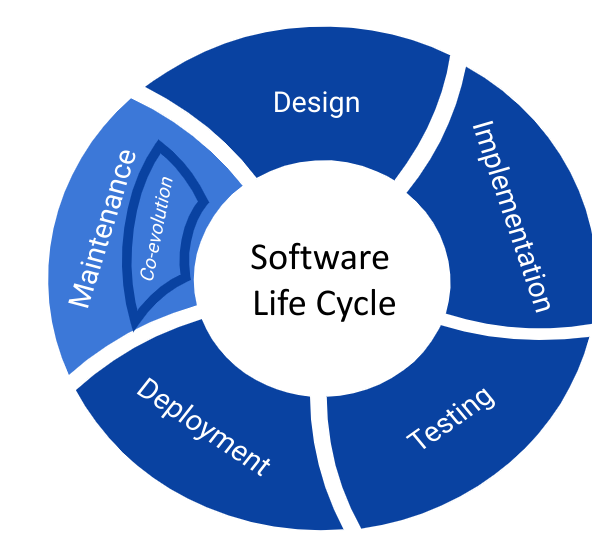
\includegraphics[width=0.6\linewidth]{./pics/soaPics/solicy.png}
	\end{center}
	\caption{Software Life Cycle}
%	{\footnotesize Titre plus long avec des explications.}
	\label{fig:softwarelifecyle}
\end{figure}

\begin{figure}[htbp]
	\begin{center}
		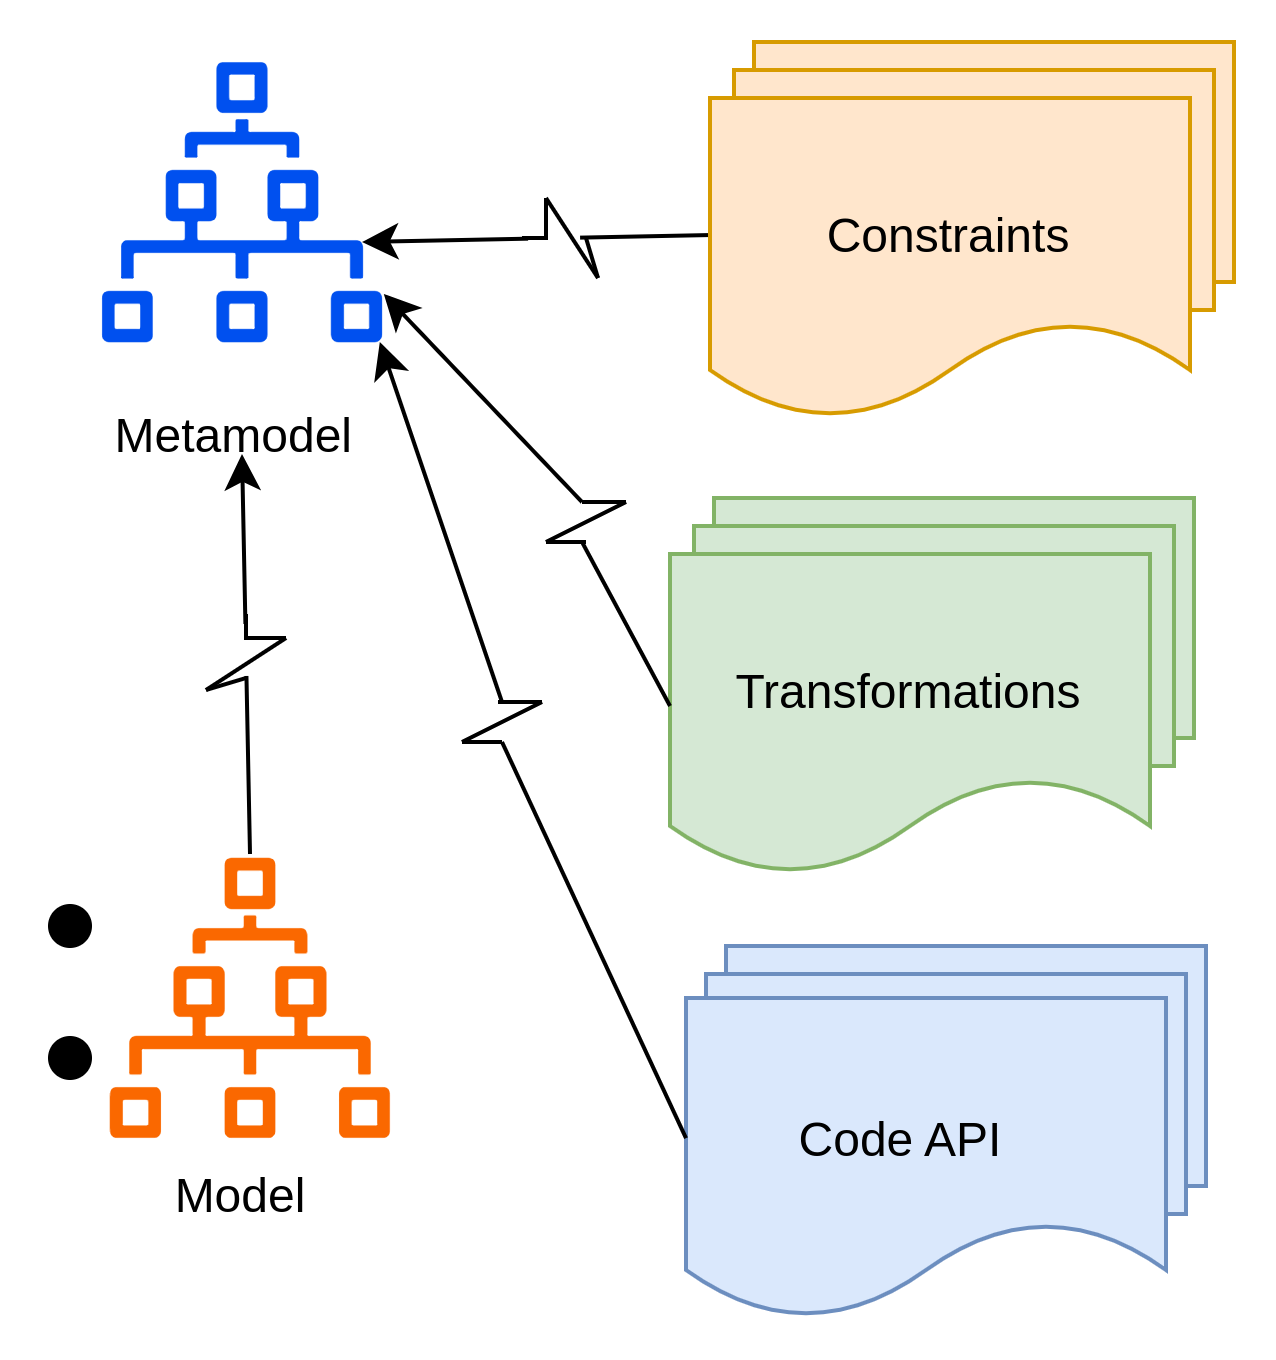
\includegraphics[width=0.6\linewidth]{./pics/soaPics/mdeecosystem.png}
	\end{center}
	\caption{MDE Ecosystem}
%	{\footnotesize Titre plus long avec des explications.}
	\label{fig:mde_ecosystem}
\end{figure}


%definition
\chapter{State Of The Art}

\chaptermark{State Of The Art}
%offline and online process
In this chapter, we present an overview of what has been done in the field of code co-evolution in the context of Model-Driven Engineering. We split this overview into ? parts. In section ?, we present the metamodel change detection approaches. Section ? presents the co-evolution of model, transformations, constraints with evolving metamodel. In section ?, we discuss code co-evolution and relevant literature about API-client evolution, language evolution, and evolution in low-code platforms. We finish this chapter with a discussion focused on limitations and research gap.
 \section{Metamodel change detection}
 One of the intrinsic properties of software artifacts is its continuous evolution~\cite{mens2008introduction}. Like any software artifact, metamodels are meant to evolve to meet the represented domain. %one key sentence of the context
 In this thesis, our context is triggered by the metamodel evolution, that's why we find essential to understand this evolution in detail.
 %metamodel diffing
 A lot of work has been done on metamodel diffing.
 Detection approaches can be classified into two main categories; online\footnote{Offline approaches perform detection after the metamodel has been evolved.} detection approaches, and offline\footnote{Online approaches perform instant detection for each change during the metamodel evolution} detection approaches. Thid classification can be refined using some factors : automation degree, types of detected changes, considered issues (overlap, indefinit length, hidden changes, order of changes, and undo operations)\cite{hebig2016approaches}.
 
 
 
  In another hand, many of them classified the detected changes based on their impact on the treated artifact (models, constraint, transformation, and code). Here we put the largest set of changes types, later, we will specify treated types with their possible impact on the code.
 
 
 Two types of evolution changes are considered when evolving a metamodel: \emph{atomic} and \emph{complex} changes~\cite{hebig2016approaches,Herrmannsdoerfer2011}. 
 Atomic changes are additions, removals, and updates of a metamodel element. Complex changes consist of a sequence of atomic changes combined together~\cite{vermolen_reconstructing_2012},~\cite{khelladi2015detecting}. For example, move property is a complex change where a property is moved from a source class to a target class. This is composed of two atomic changes: delete property and add property~\cite{Herrmannsdoerfer2011}. 
 Many approaches in the literature~\cite{Alter2015, williams2012searching,cicchetti_managing_2009,langer_posteriori_2013,vermolen_reconstructing_2012,Khelladi2016,bettini2022executable} exist to detect metamodel changes between two versions.
  
 \vspace{1em}
 	\begin{tabular}{ |c|c| } 
 		\hline
 		Type  & Change name \\
 		\hline
 		\multirow{4}{4em}{ Atomic changes} & Delete class  \\ 
 		& Delete property \\ 
 		& Add class \\ 
 		& Add property \\ 
 		& Rename class \\ 
 		& Rename property \\ 
 		& Generalize property \\ 
 		\hline
 		\hline
 		\multirow{5}{4em}{Complex changes} & Move property \\ 
 		& Push property  \\ 
 		& Pull property\\ 
 		& Inline class\\
 		& Change property type\\
 		\hline
 		
 	\end{tabular}
 	  
 	\vspace{1em}
 	
 In Model-Dricen Engineering area, metamodel changes can be divided into three categories\cite{gruschko2007towards}:
 \begin{itemize}
 	
 \item	Non-breaking changes can be resolved automatically.
  \item Breaking and resolvable changes break the conformance of existing data, although they can be automatically adapted.
 \item Breaking and unresolvable changes break the conformance of existing data, that cannot be automatically adapted, and require user intervention
 \end{itemize}
 	In API evolution context, API changes can be classified as Non-breaking API Changes	or Breaking API Changes. A breaking change is not backwards compatible. In this case, client code calling the evolved API by a Breaking Change fails to compile or may behave differently at runtime. A non-breaking change is backwards compatible. This kind of changes aims to extend the functionalities or fix errors \cite{dig2006apis}.
 \section{Co-evolution of models, constraints, and transformation}
 In MDE ecosystem, the metamodel is the starting point to have other artifacts that we defined in section ?. in this section, we will present an overview of the existing work about these artifacts co-evolution. Note that if the solution is applied during the evolution of the metamodel, we call it an online solution, otherwise it is offline.
 The comparison, advantages, and drawbacks of the presented approaches is out of the scope of this dissertation.
 
\subsection{Metamodel and model co-evolution}
Due to metamodel evolution, the model becomes "no conform". A set of resolutions are applied to co-evolve the model to gain again its conformity to the metamodel.
%change order, resolution order
%Once the metamodel changes are detected, using one of the previously presented approaches in Section ?, 
 %a set of resolutions are applied to co-evolve the model to gain again the conformity to the metamodel.
 %change order, resolution order
 The co-evolution between metamodel and models can be processed manually but it requires a huge expertise, and when the number of models to co-evolve increases, manual co-evolution becomes hard task. 
 Most of automatic and semi-automatic Co-evolution  approaches use automatic or manual diffing metamodel approaches in their solutions. Model co-evolution approaches that we found can be categorized into five categories \cite{Hebig2017}. The first category is Resolution Strategy Languages that specifies in a transformation language how to update the model given the list of metamodel changes \cite{10.1007/978-3-540-87875-9_44,sprinkle2004domain,wimmer2010using,10.1007/978-3-642-30476-7_13,10.1007/978-3-642-38883-5_10,10.1007/s10270-012-0313-5,10.1007/s10270-012-0296-2}. The category Resolution Strategy Generation groups approaches that generate full or partial resolution for each metamodel change \cite{del2007semi,de2008generating,garces2009managing,meyers2011generic,anguel2014using}.
 
 
 The third group of "Predefined Resolution Strategies" contains approaches that provide automation, when it is possible, by applying predefined resolution strategies \cite{hossler2005coevolution,florez2012coevolution,fernandez2013adapting,wachsmuth2007metamodel,cicchetti2009managing,van2011generic,becker2007process,herrmannsdoerfer2009operation,wittern2013determining}. 
 
 %We find three categories of metamodel and model co-evolution approaches.% Approaches based on resolution strategy languages that propose transformation languages created given the metamodel changes. The second category groups Resolution strategy generation approaches that allow to generate full or partial resolutions for each metamodel change.
 
  Some of these approaches requires the user intervention to make decision on the selected operation to adapt the model.
  The fourth category of Resolution strategy leaning that adopt machine learning algorithm to select the resolution strategy for metamodel changes.\cite{anguel2013towards}.%TODO Look for full paper
 
The fifth and last category is called Constrained Model Search. It groups approaches that do not use the metamodel change, but uses the original model and the new metamodel to apply a constrained-based search of valid model variants \cite{demuth2016co,gomez2014approach,schonbock2014care}. Other approaches consider the model co-evolution problem as an optimization one that does not need the list of changes of the metamodel \cite{kessentini2016automated,kessentini2019automated,kessentini2020interactive}.
%Demuth el al. [6] who used it for models co-evolution.
% There are also approaches for semi-automatic co-evolution of models that rzquires the user intervention to make decision on the selected operation to adapt the model.

%\cite{kessentini2018integrating,kessentini2019automated,cicchetti2008automating,herrmannsdoerfer2009cope,garces2009managing,wachsmuth2007metamodel},
\subsection{Metamodel and constraints co-evolution}
Another artifact that depends on the metamodel and needs to be adapted to the evolution of its metamodel is Constraints.
 Constraints co-evolutions that we can find in literature may be online \footnote{Online approaches perform instant co-evolution for each change during the metamodel evolution} or offline \footnote{Offline approaches perform co-evolution after the metamodel has been evolved.}. Every approach has its own co-evolution mechanism that treats specific types of metamodel changes and has its automation degree. Demuth et al. \cite{10.1007/978-3-642-41533-3_18} proposed a template-based, hat cannot cover all changes types, of the predefined structure of the updated constraint. Markovich et al. \cite{markovic2008refactoring} proposed refactoring rules that depends on the impact of UML class diagram evolution on the constraints. Hassam et al. \cite{hassam2011assistance} propose METAEVOL, based on a transformation language.Kusel et al \cite{kusel2014systematic} propose a solution for the co-evolution of the constrain body and do not include its context that may need co-evolution also.
 Cabot et al \cite{cabot2004automatic} treats OCL constraints co-evolution due to metamodel deletion change. Khelladi et al \cite{khelladi2017semi} proposed an approach that record the metamodel atomic and complex changes in a chronological order then apply one or many resolutions to co-evolve the constraints. Batot et al. \cite{8101267} tackles the constraint co-evolution problem as  an multi-objective optimization problem and apply heuristic-based recommendation approach that does not require/use a predefined set of transformation rules/resolutions to co-evolve the constraints. Demuth, markovitch, cabot \cite{10.1007/978-3-642-41533-3_18,markovic2008refactoring,cabot2004automatic} their approaches ar fully automatic while Hassam, kusel and Khelladi, and Batot \cite{hassam2011assistance,kusel2014systematic,khelladi2017semi,8101267} propose semi-automatic approaches since the user must select from the recommended output constraints. 
 
 
\subsection{Metamodel and transformations co-evolution}

Almost all the existing transformation approaches that we find in literature start by analyzing the impact of the metamodel on the model transformations.
Mendez et al. \cite{mendez2010towards}, Ruscio et al. \cite{di2011needed}, Garces et al.\cite{garces2014adapting}, Kusel, et al.\cite{kusel2015consistent}, and khelladi et al. \cite{khelladi2018change} proposed to co-evolve impacted transformations with a set of resolutions. The approach of khelladi et al. \cite{khelladi2018change} covers the largest set of possible resolutions where Ruscio et al. \cite{di2011needed}, estimate the cost of the co-evolution to decide about the co-evolution,they further explored the variability of the co-evolution due to the possible alternative resolution. Garcia et al.\cite{garcia2012model} proposed a ATL transformation-based approach which means that their resolutions are ATL transformations. All the approaches propose unique resolution to co-evolve each transformation.
Ruscio et al. \cite{di2011needed} approach allows developers to manually replace or refine a resolution. Khelladi et al. \cite{khelladi2018change}  allow to compose existing resolutions into a new one. Kessentini et al. \cite{kessentini2018automated} used a different approach that do not use the changes of the metamodel as input and do not process by an impact analysis, but it uses a search-based approach that relied on multi objective heuristic algorithm NSGA-II.
 \section{Code co-evolution}
 We divided the related work to code co-evolution  into four (4) main categories : 1) Metamodel and code co-evolution, 2) API and client code co-evolution, 3) Automatic Program repair, and 4) Consistency checking. 
 \subsection{Metamodel and code co-evolution}
 Co-evolution of code is distinguished from the co-evolution of other artifacts by the fact that $one$ change in a metamodel element will affect $n$ different code elements, in contrast to a $one$ to $one$ impact relationship between metamodel elements and models, constraints and transformation elements~\cite{kessentini2018integrating,kessentini2019automated,cicchetti2008automating,herrmannsdoerfer2009cope,garces2009managing,wachsmuth2007metamodel,batot2017heuristic,khelladi2017semi,correa2007refactoring,kessentini2018automated,khelladi2018change,garces2014adapting,10.1007/978-3-642-36089-3_9,kusel2015consistent,kusel2015systematic}.
 
 Yu et al.~\cite{yu2012maintaining} proposed to co-evolve the metamodels and the generated API in both directions. However, they do not co-evolve the code on top of it.% which our approach does. 
 %
 Khelladi et al.~\cite{Khelladi2020} proposed an approach that propagates metamodel changes in the code as a co-evolution mechanism. However, it is based on static analysis to detect the impacts and not on the actual errors that appear from the compilation of the code after the metamodel evolution. It further applies a semi-automatic co-evolution requiring developers' intervention, and without checking behavioral correctness with tests with no comparison to a baseline. 
 
 
 %%%%%%%%%%%%%%%%%%%%%%%%%%%%%%%%%%%%%%%%%%%%%%%%%%%%%%%%%%%%%%%%%%%%%%%%%%%%%%%%%%%%%%
 \subsection{API and client code co-evolution}
 \label{API_evolution}
 
 %In this paper, we focus so far the co-evolution on the direction metamodel to code, which is not trivial. 
 
 Existing approaches for code migration are related to our work.% We focus on the main existing approaches to compare them with our approach.
  Henkel et al.~\cite{henkel2005catchup} proposed an approach that captures refactoring actions and replays them on the code to migrate. However, they support only the changes renames, moves, and type changes. 
 
 Nguyen et al. \cite{nguyen2010graph} also proposed an approach that guides developers in adapting code by learning adaptation patterns from previously migrated code. Similarly, Dagenais et al.~\cite{dagenais2011recommending,5070565,10.1145/1932682.1869486} also use a recommendation mechanism of code changes by mining them from previously migrated code. 
 %
 Anderson et al.~\cite{andersen2010generic} proposed to migrate drivers in response to evolutions in Linux internal libraries. It identifies common changes made in a set of files to extract a generic patch that can be reused on other code parts. Gerasimou et al. \cite{10.1145/3194793.3194798} extract a set of mapping rules and apply code-based transformations to update its clients.
 // Survey about Library evolution \cite{10043250}
 %todo Coccinelle http://coccinelle.lip6.fr/
 
% 

\begin{table*}[t]
\centering
\caption{Related work comparison (to position )} 
\label{table:relatedWorkTable}
	\resizebox{16cm}{!} 
{\normalsize
\begin{tabular}{l|l|l|c|c|c|c}%|l|l|l|l|l|l|l|}
%\hline
\toprule 
 Approaches &Category & Approach & Automation & \begin{tabular}[c]{@{}c@{}}Requires \\ pre-learning\end{tabular}& Change types & Validation  \\ \midrule
 
\multicolumn{1}{l|}{ \textbf{Lamothe et al. \cite{9079197}}} & \multirow{2}{*}{} & \multirow{3}{*}{} &Semi-automatic &Yes $\checkmark$  &  \begin{tabular}[c]{@{}l@{}} Encapsulate, Move method,Remove parameter,\\Rename, Consolidate, expose implementation,\\ add contextual data,change type,\\ Replaced by exeternal API  \end{tabular}  & No $\times$  \\ \cmidrule{1-1} \cmidrule{4-7} 

\multicolumn{1}{l|}{\textbf{Fazzini et al. \cite{10.1145/3387905.3388608}} } &   \begin{tabular}[c]{@{}l@{}}Android api \\migration\end{tabular} &    \begin{tabular}[c]{@{}l@{}} Identifying migration patterns and \\rank them to select the most context-similar  \end{tabular}    & Fully-automatic& Yes $\checkmark$    &\begin{tabular}[c]{@{}l@{}}Any change in AST level\\ ( Insert/Move/Update/Delete)\end{tabular} &Yes $\checkmark$  \\ \cmidrule{1-2} \cmidrule{4-7} 

\multicolumn{1}{l|}{\textbf{Meng et al. \cite{10.5555/2486788.2486855}}} &   \begin{tabular}[c]{@{}l@{}}Bug fix \\context \end{tabular}              &          &  Semi-automatic& Yes $\checkmark$   & \begin{tabular}[c]{@{}l@{}}Any change in AST level\\ ( Insert/Move/Update/Delete)\end{tabular}& No $\times$ \\ \midrule

\multicolumn{1}{l|}{ \textbf{ Wu et al. \cite{6062100}}} & \multirow{4}{*}{} &    \begin{tabular}[c]{@{}l@{}} Hybrid approach using call \\ dependency graph and textual similarity   \end{tabular}                 
& Semi-automatic
&No $\times$ 
&\begin{tabular}[c]{@{}l@{}} change rules  :\\ One-to-One, One-to-Many \\ Many-to-One, Simple-Deleted  \end{tabular}      
& No $\times$ \\ \cmidrule{1-1} \cmidrule{3-7} 

\multicolumn{1}{l|}{\textbf{ Dagenais et al. \cite{dagenais2011recommending,5070565}}} 
&                   
&  \begin{tabular}[c]{@{}l@{}}     Recommendation approach for \\ compilation errors' correction     \end{tabular}            
& Semi-automatic
& Yes $\checkmark$ 
& Deleted or deprecated methods 
& No $\times$ \\ \cmidrule{1-1} \cmidrule{3-7} 

\multicolumn{1}{l|}{\textbf{ Henkel et al. \cite{henkel2005catchup}}} 
&      \begin{tabular}[c]{@{}l@{}} Java library \\evolution  \end{tabular}        
&   \begin{tabular}[c]{@{}l@{}}  Catch refactoring operations during \\ the API revolution the API user can replay \\ these operations later \end{tabular}     
& Semi-automatic
& Yes $\checkmark$
& \begin{tabular}[c]{@{}l@{}}     Refactoring operations: Rename Type, \\Moving Java Elements, Move static member,\\ Change Method Signature, \\ Rename non-virtual method,\\ Rename non-virtual method,\\ Rename virtual method,\\change type, rename field,\\ Use super-type where possible,\\ Introduce factory  \end{tabular}   
&  No $\times$ \\ \cmidrule{1-1} \cmidrule{3-7} 

\multicolumn{1}{l|}{\textbf{ N. Guyen et al. \cite{10.1145/1932682.1869486}}} 
&                  
&  \begin{tabular}[c]{@{}l@{}}    Recommendation approach for API \\ usage adaptation in client      \end{tabular}        
& Semi-automatic
& Yes $\checkmark$ 
& \begin{tabular}[c]{@{}l@{}}Any change in AST level\\ ( Insert/Move/Update/Delete)\end{tabular} 
&   No $\times$\\ \cmidrule{1-1} \cmidrule{3-7} 

\multicolumn{1}{l|}{\textbf{ Zhong et al. \cite{10.1145/3597503.3639084}}} 
&                  
&  \begin{tabular}[c]{@{}l@{}}    Compiler-directed tool for\\ migrating API callsite of client code     \end{tabular}        
& Fully-automatic
& no $\checkmark$ 
& \begin{tabular}[c]{@{}l@{}} N/a \end{tabular} 
&   No $\times$\\ \midrule
     
         
\multicolumn{1}{l|}{\textbf{Gerasimou et al. \cite{10.1145/3194793.3194798}}} 
&  \begin{tabular}[c]{@{}l@{}}  Other library \\Evolution  \end{tabular}  
&  \begin{tabular}[c]{@{}l@{}}   Code-based transformation to \\update client code          \end{tabular}          
&  Semi-automatic
& No $\times$
& A set of mapping rule
& No $\times$ \\ \cmidrule{1-1} \cmidrule{3-7}


\multicolumn{1}{l|}{\textbf{ Xu et al. \cite{8813263}}} 
&    \multirow{-2}{*}{}     
&  \begin{tabular}[c]{@{}l@{}}    Mining stored database edits to select \\ applicable edits  to  be reviewed        \end{tabular}                  
& Fully-automatic
& Yes $\checkmark$ 
& \begin{tabular}[c]{@{}l@{}}Any change in AST level\\ ( Insert/Move/Update/Delete) \\ classified into 3 categories : \\Single statement, Block of statements,\\ MultiBlock of statements\end{tabular} 
&   No $\times$\\ \midrule

%\multicolumn{1}{l|}{\textbf{Ochoa et al. \cite{10.1145/3510455.3512783}}}&          Maven libraries        &  \begin{tabular}[c]{@{}l@{}}     Breaking changes analysis followed \\by Impact analysis in the client*         \end{tabular}              &  & &  \CIRCLE& \\ \midrule

\multicolumn{1}{l|}{\textbf{Khelladi et al. \cite{Khelladi2020}}} 
& \multirow{2}{*}{\cellcolor{CellColor1} Model-centric} 
&                 Impact propagation approach  
&   Semi-automatic
&   No $\times$
& See Table  \ref{table:ResolutionsCatalog}
& No $\times$  \\ %\cmidrule{1-1} \cmidrule{3-7} 

\hhline{=|~|=====}


\multicolumn{1}{l|}{\cellcolor{CellColor1} Our approach   } & \cellcolor{CellColor1}   evolution              &  \cellcolor{CellColor1}    \begin{tabular}[c]{@{}l@{}}Code co-evolution guided by Metamodel \\changes pattern matching    \end{tabular}    &  \cellcolor{CellColor1} Fully-automatic  & \cellcolor{CellColor1} No $\times$  &  \cellcolor{CellColor1} See Table \ref{table:ResolutionsCatalog} & \cellcolor{CellColor1}Yes $\checkmark$ \\ \bottomrule

% &  \cellcolor{CellColor1} \CIRCLE & \cellcolor{CellColor1}  &  \cellcolor{CellColor1}\CIRCLE & \cellcolor{CellColor1}\CIRCLE \\ \bottomrule
\end{tabular}
}

\end{table*}
 
 %Our current work distinguishes from these code migration approaches~\cite{henkel2005catchup,nguyen2010graph,dagenais2011recommending,andersen2010generic,10.1145/3194793.3194798} by considering and reasoning on the changes at the metamodel level to match the different pattern usages of the generated code elements. 
 %and not at the code level. Thus, our approach treats way less changes to identify the impacted parts in the code than code migration approaches \cite{henkel2005catchup,nguyen2010graph,dagenais2011recommending,andersen2010generic}. 
% This is possible thanks to the abstraction offered by the metamodels. 
 %Whereas our work considers $one$ change of a given element, $n$ changes must be considered in order to fully migrate the code. 
 %
 % our approach VS api migration approaches
 % \cite{henkel2005catchup,andersen2010generic} 
% Moreover, there are similarities with migration approaches, %(example-based approaches and code transformation based approaches) in the aim, 
% which is evolving the dependent client code. But these approaches do not handle all the equivalents of the impacting metamodel changes we do (see Table~\ref{table:ResolutionsCatalog}), and that occurred in our case studies. They handle only a subset of changes~\cite{henkel2005catchup,andersen2010generic}. %The second main difference between our approach and the example-based approaches is that we don't use a pre-collected examples to learn how to evolve the additional code/\red{client}, we update the impacted parts of the additional code/\red{client} using only the set of detected metamodel changes \cite{6606596,9079197}. The main difference between our approach and code transformation based approaches is that they start by detecting the usages of the API, then they migrate the usages using a mapping between the old and the new version of the API. Our approach starts by detecting the changes of the metamodel then locating the impacted code before evolving it \cite{8443580}. The last main difference is that we validate our approach using test suites. Many other approaches don't treat validation step \cite{4814159}.
 %
 %Therefore, we did not consider them as a baseline because we know a priori that too many changes would not be treated, hence, the comparison would be unfair and biased. %Moreover, we used EMF for the implementation and the valuation, but our approach conceptually remains valid for other abstracted models that affect a Java code, such as in JHipster or OpenAPI.
 Other migration approaches~\cite{6606596,10.1145/3387905.3388608,9079197} rely on pre-collected examples to learn how to evolve the additional client code. Xu et al. \cite{8813263} instead of learning from code examples, it constructs a database of edits to use during clients' migration. %Our approach starts by detecting the changes of the metamodel and then locating the impacted code before co-evolving it without the need to learn from previous examples. 
 
 %Zhong et al. \cite{10.1145/3597503.3639084} propose "LibCatch", a compiler-directed tool for migrating API callsite of client code. LibCatch uses compiling error message to match it with an error type. Each error type has several corresponding migration actions to resolve the error. Then, it follows an optimization algorithm to find the right migration action to apply that minimizes the total number of compiling errors.
 
 Zhong et al. \cite{10.1145/3597503.3639084} proposes "LibCatch", a tool to co-evolve client code to APIs evolution by reducing the compilation errors. They do not consider the API changes to correctly propagate them to the code, which may lead to only eliminating the code errors while they could be incorrect resolutions, as shown in our RQ3. They further do not use any mechanism to check the behavioral correctness of the code co-evolution and with not comparison to a ground-truth.
 
 
 %\blue{Here summarize quickly the table 9}
 %To summarize, our approach overcomes the following limitations of existing approaches:
 %\begin{itemize}
 %   \item No approach can automatically co-evolve the code without learning previously from exiting examples.
 %   \item Using change interface to detect the metamodel changes which allows handling any change type.
 %   \item Only Fazzini et al. \cite{10.1145/3387905.3388608} propose to check the code migration using differential testing but it still needs previous example-based learning to update the client code.
 %\end{itemize}
 
 
 
 %%%%%%%%%%%%%%%%%%%%%%%%%%%%%%%%%%%%%%%%%%%%%%%%%%%%%%%%%%%%%%%%%%%%%%%%%%%%%%%%%
 
 
 \subsection{Automatic Program Repair}
 \label{APR}
 
 In addition to migration approaches, extensive state of the art exists on program repair~\cite{goues2019automated,liu2020efficiency,monperrus2018automatic,gazzola2017automatic}. However, they do not repair code errors, but rather bugs that are found due to failing tests (e.g., Meng at al.~\cite{10.5555/2486788.2486855}). 
 They could be used as a next step after o co-evolution. 
 
 //To refresh new references

 %Table~\ref{table:relatedWorkTable} 
 %summarizes closely related work from the metamodel and code co-evolution~\ref{metamodel_artifacts}, API-client code co-evolution~\ref{API_evolution}, and Automatic Program Repair~\ref{APR} categories. Moreover, it compares and highlights the advantages of our approach over those related work. In particular, we compare them with the following criteria: %selected the comparison features as follows : 
 
 %\begin{enumerate}
 	%\item Category: it represents the evolved artifact impacting the code.
 	%\item Approach: it gives the main idea of the approach.
 %	\item Automation: it indicates whether the approach is automatic, semi-automatic, or manual.
 %	\item "Requiring pre-learning": %many approaches need to analyse supplementary data to be capable of co-evolving the code. 
 %	this feature indicates if a given approach is standalone by immediately co-evolving the code or needs previous external code analysis to learn how to co-evolve client code by synthesising the co-evolution pattern.
 %	\item Changes types: it conveys the changes handled by each approach.
 %	\item Validation: to ensure that the co-evolution did not impact the behavior of the code, a post validation step can be added. This feature indicates if the approach uses any mean of checking behavioral correctness of the code after the co-evolution.
% \end{enumerate}
 
% From Table~\ref{table:relatedWorkTable}, we observe that only two existing approaches are fully automatic and all the rest are semi-automatic. Only three approaches are standalone without requiring a pre-learning phase before the co-evolution. Our approach is fully automatic and standalone. Moreover, several different set of changes are handled by each approach, varying from low AST changes to high level composed (refactoring likes) changes as in Table~\ref{table:ResolutionsCatalog} in our work. Finally, only Fazzini et al.~\cite{10.1145/3387905.3388608} proposed to validate the co-evolved Android Apps with a similar methodology as in our work based on tests' execution. 
 
 \subsection{Consistency checking }
 \label{Consistency_checking}
  Close to code co-evolution, Riedl et al.~\cite{riedl2014towards} proposed an approach to detect inconsistencies between UML models and code. Kanakis et al.~\cite{kanakis2019empirical} showed that inconsistency information of model change and code error can help to resolve them in the code, which is equivalent to our matched pattern usages. 
 Pham et al.~\cite{pham2017bidirectional} proposed an approach to synchronize architectural models and code with bidirectional mappings.
 %
 Jongeling et al.~\cite{jongeling2020towards} proposed an early approach for the consistency checking between system models and their implementations by focusing on recovering the traceability links between the models and the code. Jongeling et al.~\cite{jongeling2022Structural} later rely on the recovered traces to perform the consistency checking task.  %https://www.es.mdh.se/pdf_publications/5848.pdf
 %
 Zaheri et al.~\cite{zaheri2021towards} also proposed to support the checking of the consistency-breaking updates between models and generated artifacts, including the code. However,~\cite{pham2017bidirectional,jongeling2020towards,jongeling2022Structural,zaheri2021towards} do not focus on co-evolving the code to repair the inconsistencies with the models. 
 \subsection{Language evolution}
 
Language evolution is related to  various technological spaces \cite{ivanov2002technological}. Grammars evolve in \cite{5279907}, metamodels evolve \cite{favre2003meta}, schemas evolve  \cite{lammel2001format,meyer1996schema}, ontologies evolve \cite{flouris2008ontology}, and APIs evolve \cite{dig2006apis}, too.
  
    
 There are two types of languages: General Purpose Languages (GPL) and Domain-Specific Languages(DSL).
 Programming languages are General purpose one. Their evolution consist mainly of feature additions that allows at sopme extent the stability of the code and do not break it.
 This evolution is due to two types of causes : 1) External, for example for hardware changes, the control of business needs, or the progress of scientific research. 2) Internal for bug fixing, or improving the verbosity of the language.
 Every change to a programming language API has the potential to affect programs written
 in this language. For example, Python 2 and 3 have major incompatibilities that leads to maintenance costs.
 A recent study shows that developers lack awareness of the subsequent possible incompatibilities which make code maintenance a hard task \cite{dietrich2016java}
 
Regarding programming languages evolution, many works were centered around change-impact analysis before proposing an adaptation approach \cite{arnold1996software,ren2004chianti,ryder2001change}


 
 \cite{urma2017programming} propose PytypemonitorInfer, a dynamic light-weight type inference tool for Python to automatically provide insights useful for migration about a Python program.
 few works were done for specific languages evolution, for example, Expansion and evolution of the R programming language regarding linguistic understanding of human language \cite{urma2017programming}.
 
 Regarding Domain-Specific evolution, works treated this topic from many aspects, and from different ecosystems and case studies.
  
 ref :Industrial experiences with the evolution of a DSL \cite{schuts2021industrial}
 DSL is strictly coupled to the domain and
 its requirements/capabilities at the time in which the DSL is written. If the domain requirements and/or capabilities change, then the DSL could become inadequate to deal with the changed domain.
 incrementally changed the language ()a five year old DSL) supporting multiple hardware configurations. initially prefixed later defined by the user. Domain experts no longer need DSL experts to define new configuration with new movements, states and zones.
 Ref2 :DSL/Model Co-Evolution in Industrial EMF-Based MDSE Ecosystems \cite{mengerink2016dsl}
 J.G.M.
 DSL evolves : J.-M. Favre, “Languages evolve too! changing the
 software time scale,” in Principles of Software
 Evolution, 2005, pp. 33–42.  \cite{favre2005languages}, M. Herrmannsdörfer and G. Wachsmuth, “Coupled
 evolution of software metamodels and models,” in
 Evolving Software Systems. Springer, 2014, pp. \cite{herrmannsdorfer2013coupled}
 33–63.
 that presence of inter-DSL dependencies in an MDSE ecosystem causes a ripple effect and increases costs of manual maintenance. Hence, an automatic approach is required to facilitate co-evolution of artifacts in MDSE ecosystems.
 
 ref :Language Evolution in Practice: The History of GMF ,Herrmannsdoerfer, \cite{10.1007/978-3-642-12107-4_3}
 presented a method to investigate the evolution of modeling languages
 hint at the possible effects on the related language development artifacts

 works treated the topic of dsl evolution from many aspects and from different ecosystems (case studies).
 
 ref :
 \section{Behavioral correctness of the co-evolution}
  \section{LLMs for co-evolution }
 %TODO What has been done so far: 
%TODO Change detection
%TODO Metamodel-Transformation co-evolution
%TODO Metamodel-Constraint co-evolution
%TODO Metamodel-Model co-evolution
%TODO Metamodel-code co-evolution
%Discussion about automation degree of the approaches, best in cases and other cases not really

%TODO API-Client co-evolution

%TODO Language Evolution (e.g., Java V1 to V2)
%TODO Evolution in low-code platforms
%TODO Classification of related work 

%TODO Focus on limitations/research gap.
